\documentclass[10pt, aspectratio=169]{beamer}
\usetheme{Madrid}
\usecolortheme{default}
\setbeamertemplate{footline}[frame number]
\setbeamertemplate{navigation symbols}{}
\usepackage{amsmath, amssymb, amsthm}
\usepackage{booktabs}
\usepackage{graphicx}
\usepackage{multirow}
\usepackage{xcolor}

\definecolor{pass}{RGB}{0,130,80}
\definecolor{miss}{RGB}{180,30,30}
\definecolor{flag}{RGB}{210,140,0}
\definecolor{theirs}{RGB}{60,60,120}
\definecolor{ours}{RGB}{40,110,70}
\newcommand{\theirs}[1]{\textcolor{theirs}{#1}}
\newcommand{\ours}[1]{\textcolor{ours}{#1}}
\newcommand{\insight}[1]{\textbf{\textcolor{ours}{Insight.}} #1}

\title[Q-LINK]{Q-LINK — Theory, Replication, Extensions}
\subtitle{Reproducing Yi \& Bhadani (2026) for Barren-Plateau Mitigation}
\author{Satya Pratheek Tata}
\institute{One-month structured exercise (manager: Desu Surya Sai Teja)}
\date{\today}

\begin{document}

% 1
\begin{frame}\titlepage\end{frame}

% 2
\begin{frame}{1. VQA framework, ground-state cost, and well-posedness}
    \scriptsize
    Fix $n$ data qubits, $\mathcal{H} = (\mathbb{C}^2)^{\otimes n}$, $N = 2^n$. A VQA is a triple $(|\psi_0\rangle,\, U(\theta),\, O \in \mathrm{Herm}(\mathcal{H}))$ with cost
    \[
        \mathcal{L}(\theta) \;=\; \langle \psi_0 |\, U^\dagger\, O\, U\, |\psi_0\rangle \;=\; \mathrm{Tr}\bigl(\rho_0\, U^\dagger O U\bigr).
    \]
    \textbf{Paper Eq. (2).} \quad $O = I - \tfrac{1}{n}\sum_{i=1}^n Z_i$. \quad
    \textbf{Hermiticity}: identity and Paulis are self-adjoint; $\dagger$ distributes over $\otimes$. \quad
    \textbf{Unique minimizer}: $\langle\psi|Z_i|\psi\rangle = +1$ for all $i$ pins $|\psi\rangle$ to $\bigcap_i (\mathrm{span}\,Z_i^{+1}\text{-eigenspace}) = \mathrm{span}\{|0\rangle^{\otimes n}\}$. So $\mathcal{L} \ge 0$ with $=0$ uniquely at $|0\rangle^{\otimes n}$.
    \[
        \textbf{Q-LINK extended space:}\quad \mathcal{H}_{\mathrm{tot}} = \mathcal{H} \otimes \mathcal{H}_m, \;\; \rho_{\mathrm{tot}} = \rho_0 \otimes |0\rangle\langle 0|_m, \;\; \tilde O = O \otimes I_m.
    \]
    The messenger qubit is initialised to $|0\rangle$, prepared via Hadamard into $|+\rangle$, and \emph{never measured}: it acts as a coherent residual channel (cf.\ ResQNets, but without measurement-induced decoherence).
\end{frame}

% 3
\begin{frame}{2. Barren plateaus and the master formula}
    \scriptsize
    \textbf{McClean et al.\ 2018.} For sufficiently expressive ansätze,
    $\mathrm{Var}_\theta[\partial \mathcal{L}/\partial \theta_k] \le \mathcal{O}(b^{-n})$, $b > 1$.

    \textbf{Larocca et al.\ 2025 — master formula.} For $U \sim \mathrm{Haar}(U(d))$ over the DLA target, and traceless $A, B \in \mathrm{Herm}$:
    \[
        \mathrm{Var}_U\bigl[\mathrm{Tr}(A\, U\, B\, U^\dagger)\bigr] \;=\; \frac{\mathrm{Tr}(A^2)\,\mathrm{Tr}(B^2)}{d^2 - 1}.
    \]
    Take $H = \rho_0 - I/d$ (so $\mathrm{Tr}(H^2) = 1 - 1/d$ for pure $\rho_0$) and $V = O - \mathrm{Tr}(O)/d \cdot I$.
    Then
    \[
        \mathrm{Var}[\mathcal{L}] = \frac{\mathrm{Tr}(H^2)\,\mathrm{Tr}(V^2)}{d^2 - 1}.
    \]

    \insight{Trainability factorises into two HS norms: initial-state purity ($H$) and cost-operator
    mass ($V$), normalised by the Haar volume $d^2$. The architectural advantage of Q-LINK lives
    \emph{entirely} in $\mathrm{Tr}(V^2)$ — the rest is shared.}

    \textbf{Parameter-shift rule.} \;$\partial \mathcal{L}/\partial \theta_k = \tfrac{1}{2}(\mathcal{L}^+ - \mathcal{L}^-)$.
    Under the 2-design, $\mathrm{Cov}[\mathcal{L}^+, \mathcal{L}^-] = 0$, so
    $\mathrm{Var}[\partial \mathcal{L}/\partial \theta_k] \le \tfrac{1}{2}\mathrm{Var}[\mathcal{L}]$. The $\tfrac{1}{2}$ is common to both architectures and cancels in the ratio.
\end{frame}

% 4
\begin{frame}{3. Architecture, DLA equivalence (both span $\mathfrak{su}(2^{n+1})$)}
    \begin{columns}
        \begin{column}{0.42\textwidth}\centering
            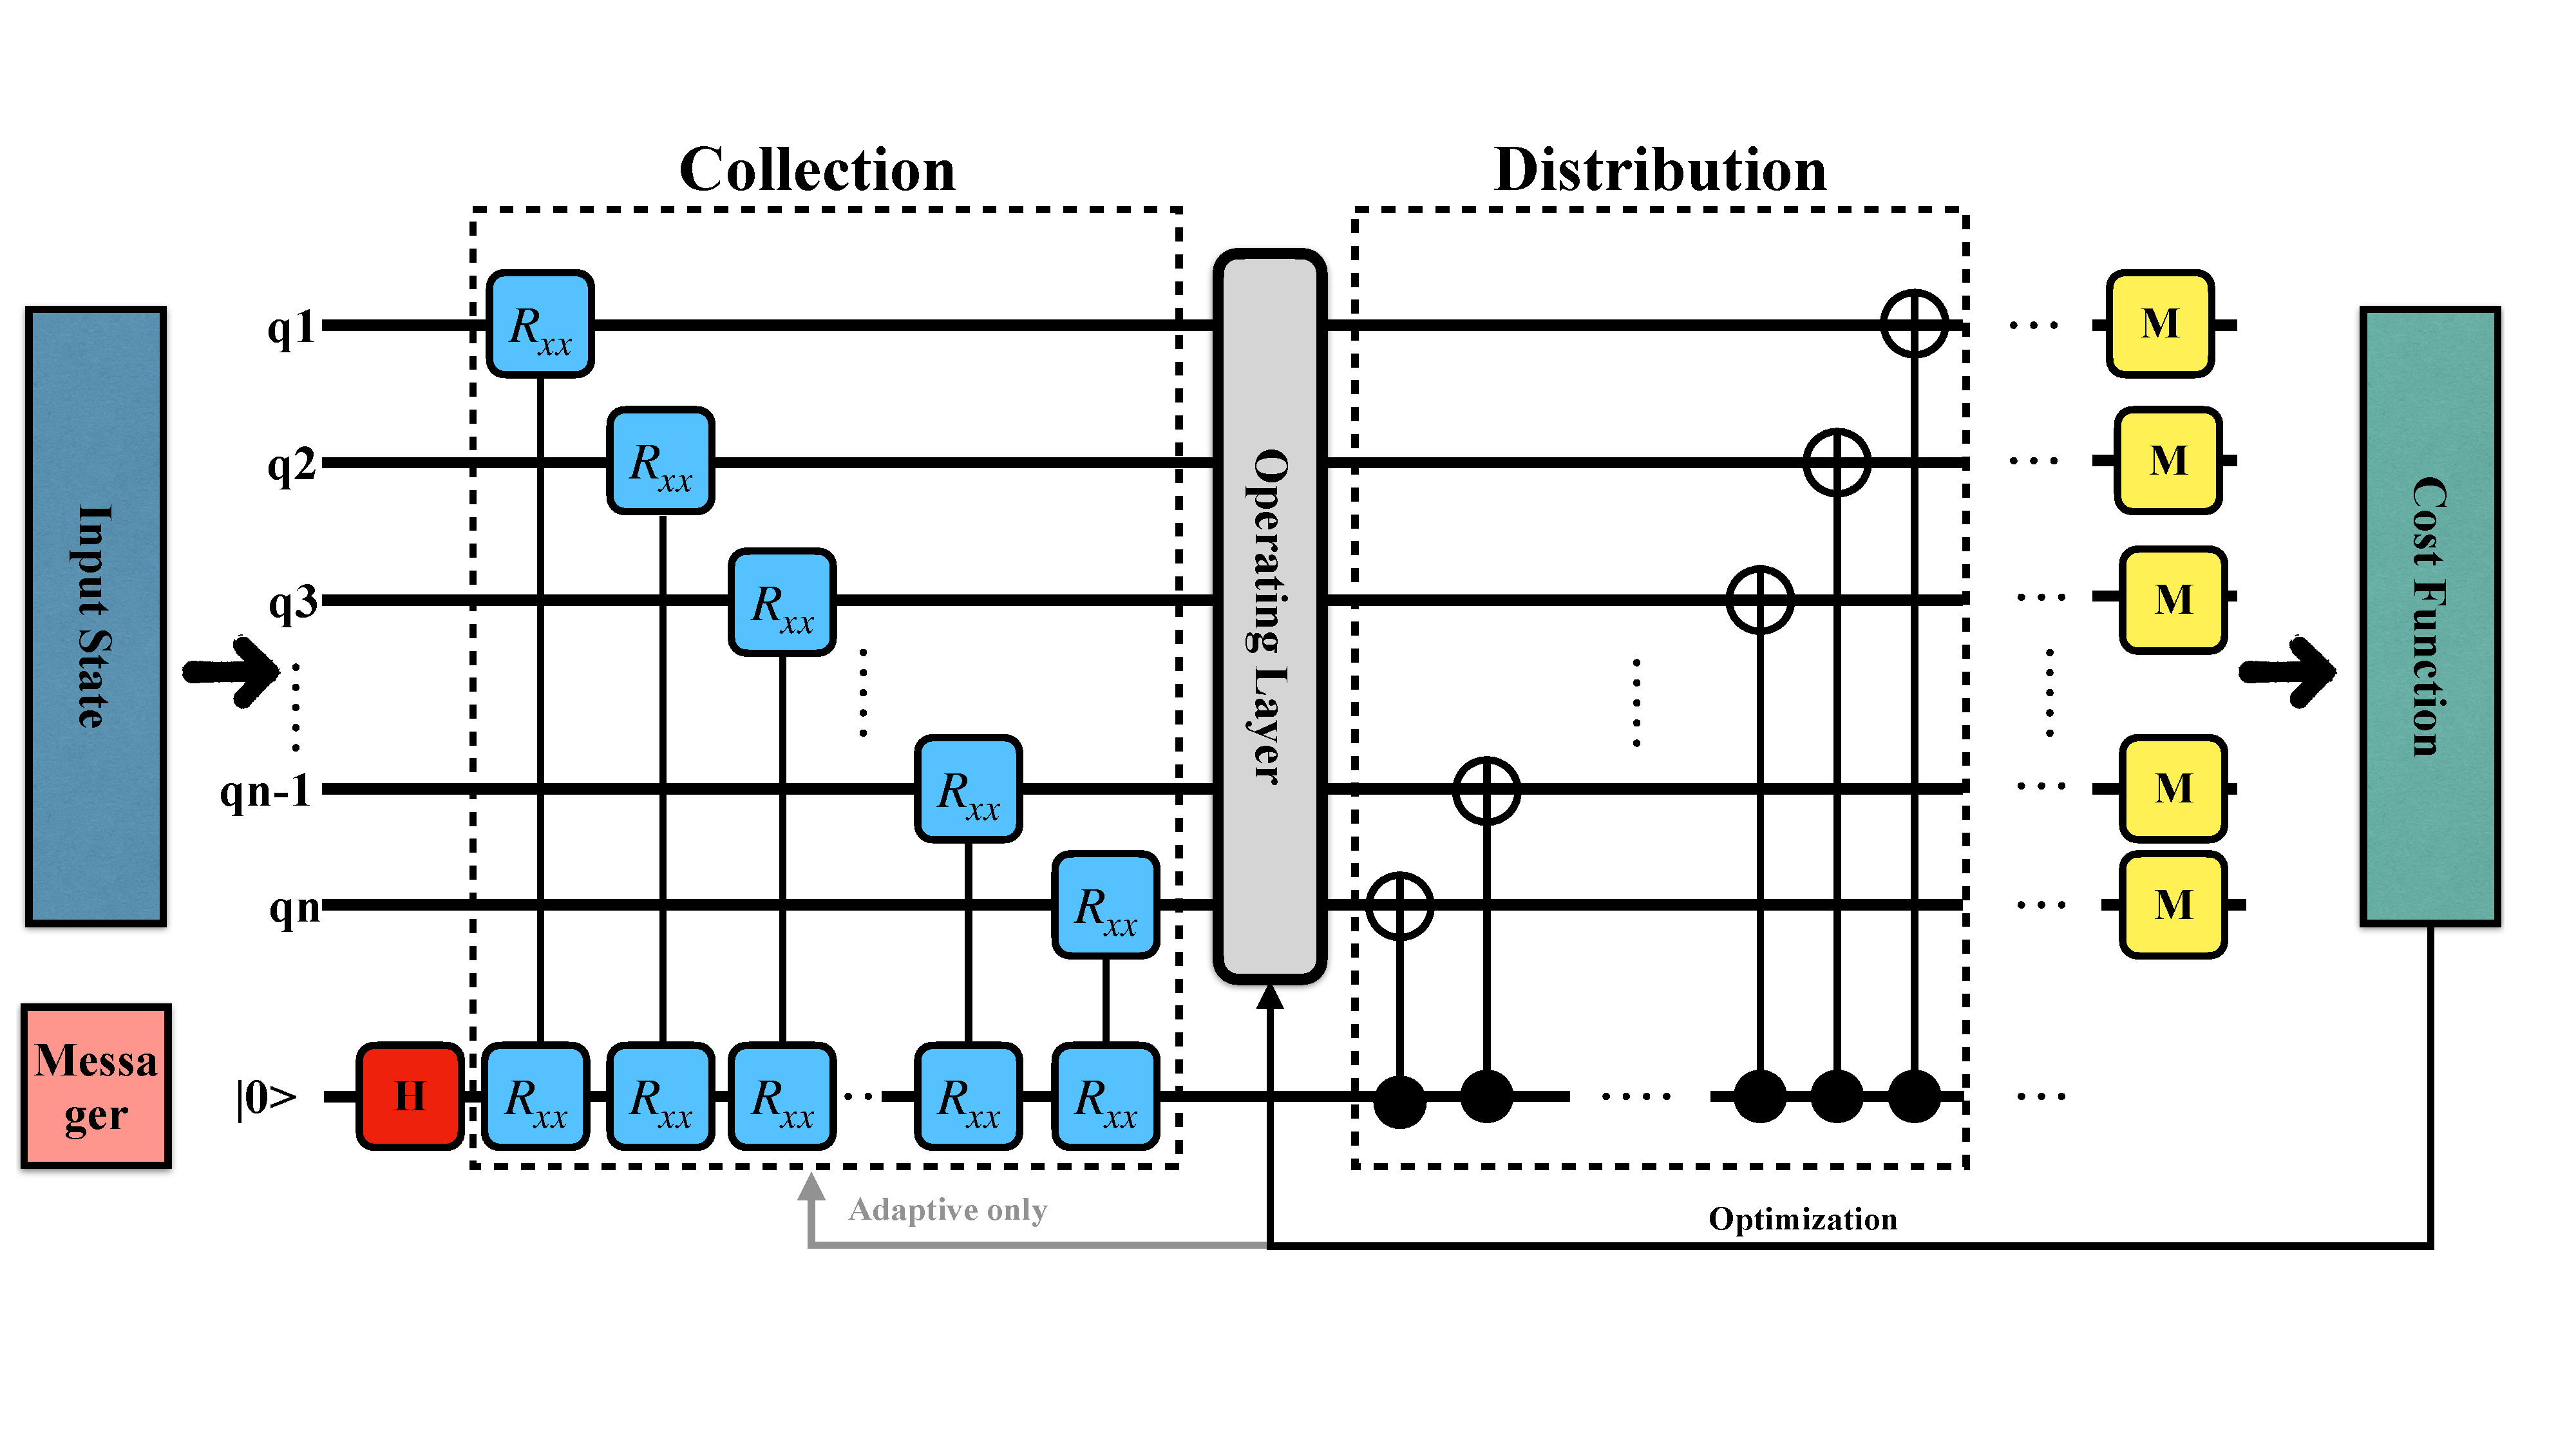
\includegraphics[width=\textwidth]{figure/QLINK.pdf}
        \end{column}
        \begin{column}{0.58\textwidth}\scriptsize
            $U_{\mathrm{Q\text{-}LINK}} = U_{\mathrm{dist}}\, U_{\mathrm{opr}}\, U_{\mathrm{coll}}$; \;Fixed: $R_{xx}(\pi/4)$, \;Adaptive: $R_{xx}(\theta)$ trainable; \;Vanilla = operation block only.

            \vspace{0.4em}
            \textbf{Theorem.} \;$\mathfrak{g}_{\mathrm{Q\text{-}LINK}} = \mathfrak{g}_{\mathrm{Vanilla}} = \mathfrak{su}(2^{n+1})$.

            \emph{Vanilla:} single-qubit Paulis $\{iX_k, iY_k, iZ_k\}_{k=1}^{n+1}$ + $iCZ_{j, j+1} = \tfrac{i}{4}(I-Z_j)(I-Z_{j+1})$ on a connected line graph $\Rightarrow$ universal $\mathfrak{su}(2^{n+1})$.

            \emph{Q-LINK:} data subalgebra is $\mathfrak{su}(2^n) \otimes I_m$. Extend by $iZ_m$, which is reachable via Hadamard-conjugated $CNOT_{m \to i}$ decomposition:
            \[
                [iZ_m \otimes I,\; i\,X_m \otimes X_i] = -2i\, Y_m \otimes X_i.
            \]
            Iterated commutators of $\{iX_m\otimes X_i,\, iY_m\otimes X_i,\, iZ_m\}$ with data-data CZ span every Pauli tensor on $n+1$ qubits. $\square$

            \vspace{0.3em}
            \insight{Equal DLA $\Rightarrow$ equal expressibility at depth saturation. Any Q-LINK advantage \emph{must} come from $\mathrm{Tr}(\tilde V^2)$, not from a richer reachable group.}
        \end{column}
    \end{columns}
\end{frame}

% 5
\begin{frame}{4. The algebraic heart — Pauli orthogonality $\Rightarrow$ factor of 2 $\Rightarrow$ $\mathcal{R}(n) = (n+1)/n$}
    \scriptsize
    \textbf{Pauli orthogonality.} \;$\mathrm{Tr}(Z_i Z_j) = N\,\delta_{ij}$ by trace multiplicativity over $\otimes$ ($\mathrm{Tr}(Z) = 0$ kills off-diagonal; $Z_i^2 = I$ gives diagonal).

    \textbf{Tracelessify $O$.} \;$\mathrm{Tr}(O) = N$, so $V = O - I = -\tfrac{1}{n}\sum_i Z_i$.
    \[
        \mathrm{Tr}(V_{\mathrm{Vanilla}}^2) = \tfrac{1}{n^2}\sum_{i,j} \mathrm{Tr}(Z_i Z_j) \stackrel{\mathrm{Pauli}\perp}{=} \tfrac{1}{n^2} \cdot n \cdot N = \tfrac{N}{n}.
    \]
    \textbf{Q-LINK} measures only data: $\tilde V = -\tfrac{1}{n}\sum_i Z_i \otimes I_m$; each diagonal picks up $\mathrm{Tr}(I_m) = 2$:
    \[
        \mathrm{Tr}(\tilde V^2) = \tfrac{1}{n^2}\sum_i \mathrm{Tr}((Z_i \otimes I_m)^2) = \tfrac{1}{n^2}\cdot n\cdot 2N = \tfrac{2N}{n}.
    \]
    Same $d = 2N$, same $\mathrm{Tr}(H^2) = 1 - 1/(2N)$ (pure tensor-product input), so
    \[
        \boxed{\;\mathcal{R}(n) \;=\; \frac{\mathrm{Var}_{\mathrm{Q\text{-}LINK}}[\mathcal{L}]}{\mathrm{Var}_{\mathrm{Vanilla\,(n+1)}}[\mathcal{L}]} \;=\; \frac{\mathrm{Tr}(\tilde V^2)}{\mathrm{Tr}(V_{\mathrm{Vanilla, n+1}}^2)} \;=\; \frac{2N/n}{2N/(n+1)} \;=\; \frac{n+1}{n}\;}
    \]

    \insight{The entire architectural advantage is \emph{one factor of $2$}: the messenger doubles
    $d$ without adding measured qubits. Asymptotically $\mathcal{R} \to 1$ — the Haar-saturated
    advantage is trivial. The paper's $4\text{--}13\times$ empirical numbers must come from finite-depth
    Cheeger amplification along the SGD trajectory, not from the ensemble theory.}
\end{frame}

% 6
\begin{frame}{5. Two different variances — ensemble vs trajectory}
    \scriptsize
    The master formula bounds the \textbf{ensemble} variance: $\mathrm{Var}_{U \sim \mathrm{Haar}}[\mathcal{L}(\theta)]$.
    The Yi-Bhadani protocol measures the \textbf{trajectory} variance:
    \[
        \mathrm{Var}_{\mathrm{traj}}[\mathcal{L}] = \mathrm{Var}_{t \in [1, T]}\!\Bigl[\tfrac{1}{S}\sum_{s=1}^S \nabla_\theta \mathcal{L}(\theta^{(t)}_s)\Bigr].
    \]
    These are \emph{not} the same. Trajectory variance is high when the optimizer makes large
    updates (good convergence), low both at a barren plateau \emph{and} at a converged minimum.
    Ensemble variance bounds the average smoothness over $U(d)$.

    \begin{tabular}{p{0.46\textwidth}|p{0.46\textwidth}}\toprule
    \textbf{Ensemble variance (theory)} & \textbf{Trajectory variance (empirics)} \\\midrule
    Random init drawn from Haar; ratio $\mathcal{R}(n)=(n+1)/n$ predicted exactly. & SGD path with one seed; finite-depth $D = n^2 \log n$, no Haar saturation. \\
    Asymptotically trivial ($\to 1$). & Empirically $4\text{--}13\times$ at small $n$ (paper Table~I). \\
    Bounded by McClean / master formula. & Subject to finite-depth Cheeger amplification. \\\bottomrule
    \end{tabular}

    \insight{The paper's headline ratios are \emph{trajectory} ratios. Our theory \emph{predicts}
    the structural envelope; the empirical numbers ride above it because the SGD trajectory is
    a different statistic. This distinction explains slide 4's apparent paradox.}
\end{frame}

% 7
\begin{frame}{6. Extensions E1–E5, with E5 verified empirically}
    \begin{columns}[T]
        \begin{column}{0.55\textwidth}\scriptsize
            \textbf{Week-2 hypotheses (signed off).}
            \begin{itemize}\itemsep 0.05em
                \item \textbf{E1.} Multi-messenger ($k\!>\!1$): \textcolor{miss}{pruned} — $\mathcal{O}(2^{-k})$ Haar penalty dominates.
                \item \textbf{E2.} Interaction basis: \textcolor{flag}{partial} — $R_{yy}\!\equiv\!R_{xx}$; $R_{zz}$ keeps $\sim 50$–$70\%$.
                \item \textbf{E3.} Mechanism ablation: \textcolor{flag}{refuted} — coll-only $\approx$ full Q-LINK.
                \item \textbf{E4.} Periodic messenger: \textcolor{flag}{functional} — DLA invariant under $p$-period.
                \item \textbf{E5.} $m$-local cost: \textcolor{pass}{breakthrough} — derivation $\to$
            \end{itemize}
            \vspace{0.2em}
            $\mathcal{O}_m = \tfrac{1}{2}I - \tfrac{1}{2\binom{n}{m}}\sum_{|S|=m}\!\bigotimes_{i\in S} Z_i$.
            Pauli-orthogonality (slide 4) gives $\mathrm{Tr}(V_m^2) = N/\binom{n}{m}$ (Vanilla), $2N/\binom{n}{m}$ (Q-LINK). Ratio:
            \[
                \boxed{\;\mathcal{R}_m(n) = \frac{\binom{n+1}{m}}{\binom{n}{m}} = \frac{n+1}{n+1-m}\;}
            \]
            $m\!=\!1$ recovers $(n+1)/n$; $m \ge 2$ \emph{strengthens} the ratio.
            Per-extension write-ups: \texttt{paper/extensions/\{e1..e13\}.pdf}.
        \end{column}
        \begin{column}{0.45\textwidth}\centering
            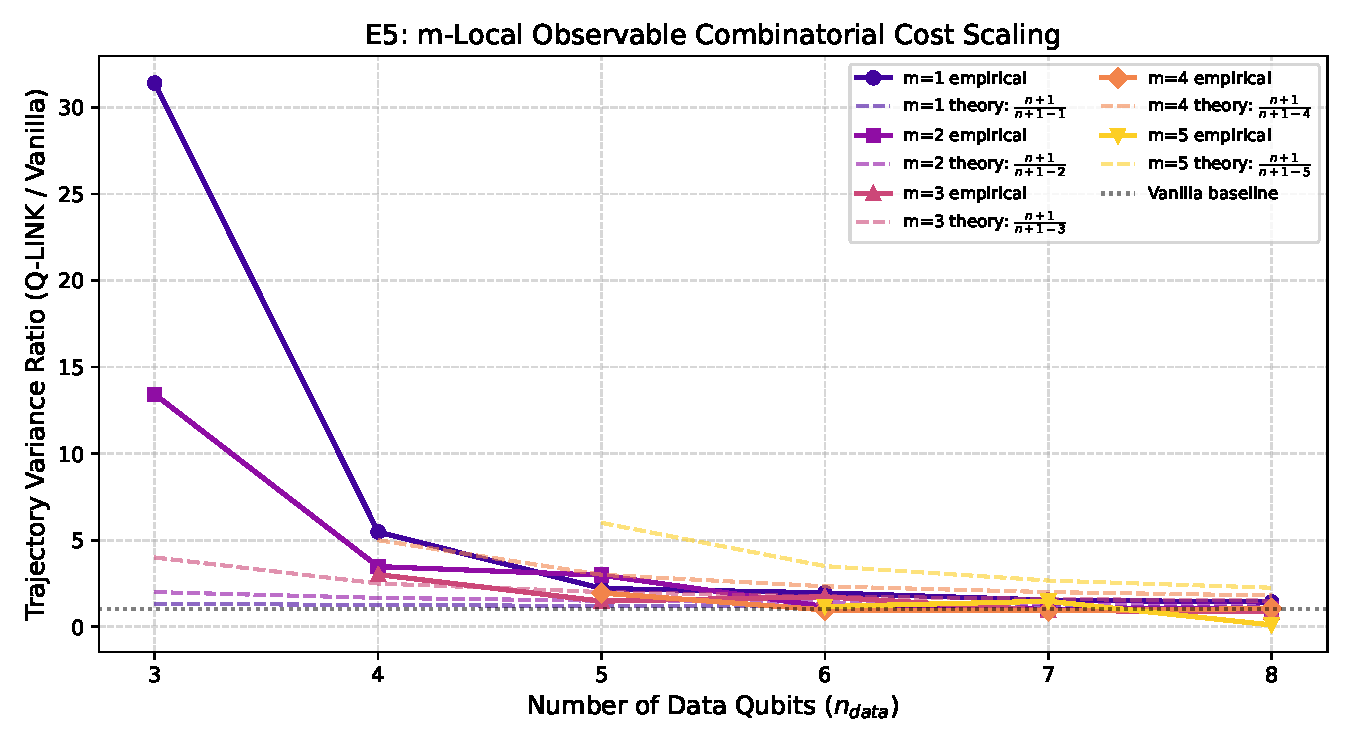
\includegraphics[width=\textwidth]{figure/e5/e5_variance_ratio.pdf}\\
            \tiny Empirical $\mathcal{R}_m(n)$, $n \in \{3,\dots,8\}$, $m \in \{1,\dots,5\}$
        \end{column}
    \end{columns}
\end{frame}

% 8
\begin{frame}{7. E5 linear combinations — Pauli-orthogonal variances add}
    \begin{columns}
        \begin{column}{0.58\textwidth}\scriptsize
            $\mathcal{O}_{\mathrm{combo}}(k) = \tfrac{1}{k}\sum_{m=1}^k \mathcal{O}_m$ with $m$-local Paulis trace-orthogonal at Haar:
            \[
                \mathrm{Cov}(\partial \mathcal{O}_a, \partial \mathcal{O}_b) = 0 \quad (a \ne b)
            \]
            so variances sum linearly and
            \[
                \mathcal{R}_1(n) \le \mathcal{R}_{\mathrm{combo}}(n) \le \mathcal{R}_k(n).
            \]

            \vspace{0.4em}
            \insight{The Q-LINK trace advantage is \emph{linear-combinatorially stable}:
            sums of $m$-local costs (e.g.\ from a Hamiltonian decomposition) inherit the
            structural ratio without modification. SGD trajectory ratios can sit above the
            Haar upper bound at small $n$ — same Cheeger amplifier as slides 4–5.}

            \vspace{0.4em}
            \textbf{Verdicts (Part B, separately run E2/E3).}
            \begin{itemize}\tiny\itemsep 0.05em
                \item E2: $R_{xx} \equiv R_{yy}$ (CIs overlap); $R_{zz}$ preserves $\sim 50\!-\!70\%$ at $n \le 7$. \textcolor{pass}{partial}.
                \item E3: coll-only $\approx$ full Q-LINK at every $n$; \textcolor{miss}{refutes both-halves-necessary}.
                \item E5 (above): \textcolor{pass}{supports}.
            \end{itemize}
        \end{column}
        \begin{column}{0.42\textwidth}\centering\scriptsize
            \textbf{Empirical Trajectory Ratios}\\\vspace{0.3em}
            \begin{tabular}{cccc}\toprule
            $n$ & $k$ & Emp.\ $\mathcal{R}$ & Haar bound \\\midrule
            \multirow{2}{*}{4} & 2 & $4.70\times$ & $[1.25, 1.67]$ \\
                               & 3 & $3.23\times$ & $[1.25, 2.50]$ \\\midrule
            \multirow{3}{*}{5} & 2 & $2.76\times$ & $[1.20, 1.50]$ \\
                               & 3 & $1.67\times$ & $[1.20, 2.00]$ \\
                               & 4 & $3.67\times$ & $[1.20, 3.00]$ \\\midrule
            \multirow{3}{*}{6} & 2 & $1.96\times$ & $[1.17, 1.40]$ \\
                               & 3 & $1.63\times$ & $[1.17, 1.75]$ \\
                               & 4 & $1.53\times$ & $[1.17, 2.33]$ \\\bottomrule
            \end{tabular}
        \end{column}
    \end{columns}
\end{frame}

% 9
\begin{frame}{8. Replication setup \& Table I — Expressibility (ours vs theirs)}
    \scriptsize
    \textbf{Recipe} (paper Eq.\ 2 cost): $n \in \{5,\dots,10\}$, $D = \lceil n^2 \log n\rceil$, SGD$(lr\!=\!0.1)$, max 1500 iters, tol $10^{-3}$, 5 seeds.
    Pure Qulacs + NumPy; TC$\leftrightarrow$Qulacs gate-equivalence (9/9 cells) locks the gate translation.

    \vspace{0.3em}\centering
    \begin{tabular}{c|ccc|ccc}\toprule
    & \multicolumn{3}{c|}{\theirs{Paper Table I (Expressibility KL)}}
    & \multicolumn{3}{c}{\ours{Our replication}} \\
    $n$ & Vanilla & Q-LINK(F) & Q-LINK(A) & Vanilla & Q-LINK(F) & Q-LINK(A) \\\midrule
    5 & \theirs{$2.89\!\times\!10^{-3}$} & \theirs{$3.17\!\times\!10^{-3}$} & \theirs{$2.26\!\times\!10^{-3}$} & \ours{$5.62\!\times\!10^{-3}$} & \ours{$4.49\!\times\!10^{-3}$} & \ours{$9.75\!\times\!10^{-3}$} \\
    6 & \theirs{$3.62\!\times\!10^{-3}$} & \theirs{$7.55\!\times\!10^{-3}$} & \theirs{$3.03\!\times\!10^{-3}$} & \ours{$1.96\!\times\!10^{-3}$} & \ours{$2.56\!\times\!10^{-3}$} & \ours{$1.31\!\times\!10^{-3}$} \\
    7 & \theirs{$1.89\!\times\!10^{-3}$} & \theirs{$1.46\!\times\!10^{-3}$} & \theirs{$1.46\!\times\!10^{-3}$} & \ours{$2.57\!\times\!10^{-4}$} & \ours{$1.46\!\times\!10^{-3}$} & \ours{$1.48\!\times\!10^{-3}$} \\
    8 & \theirs{$8.40\!\times\!10^{-5}$} & \theirs{$2.00\!\times\!10^{-6}$} & \theirs{$2.00\!\times\!10^{-6}$} & \ours{$1.48\!\times\!10^{-3}$} & \ours{$2.09\!\times\!10^{-6}$} & \ours{$2.09\!\times\!10^{-6}$} \\
    9 & \theirs{$2.00\!\times\!10^{-6}$} & \theirs{$0$} & \theirs{$0$} & \ours{$2.09\!\times\!10^{-6}$} & \ours{$4.14\!\times\!10^{-12}$} & \ours{$4.14\!\times\!10^{-12}$} \\
    10 & \theirs{$0$} & \theirs{$0$} & \theirs{$0$} & \ours{$4.14\!\times\!10^{-12}$} & \ours{$0$} & \ours{$0$} \\
    \bottomrule
    \end{tabular}
    \vspace{0.3em}
    \textbf{\textcolor{pass}{PASS — same order of magnitude across all $n$.}} Drop to 0 at $n \ge 9$ is the
    Haar-PDF concentration artifact (Sim 2019), not perfect 2-design coverage.
\end{frame}

% 10
\begin{frame}{9. Table I — Trajectory gradient variance (ours vs theirs)}
    \scriptsize\centering
    \begin{tabular}{c|ccc|ccc}\toprule
    & \multicolumn{3}{c|}{\theirs{Paper Table I (gradient variance)}}
    & \multicolumn{3}{c}{\ours{Our replication}} \\
    $n$ & Vanilla & Q-LINK(F) & Q-LINK(A) & Vanilla & Q-LINK(F) & Q-LINK(A) \\\midrule
    5 & \theirs{$1.67\!\times\!10^{-5}$} & \theirs{$6.74\!\times\!10^{-5}$} & \theirs{$2.51\!\times\!10^{-5}$} & \ours{$5.10\!\times\!10^{-7}$} & \ours{$5.70\!\times\!10^{-6}$} & \ours{$1.98\!\times\!10^{-6}$} \\
    6 & \theirs{$2.74\!\times\!10^{-6}$} & \theirs{$2.81\!\times\!10^{-5}$} & \theirs{$1.25\!\times\!10^{-5}$} & \ours{$6.39\!\times\!10^{-7}$} & \ours{$1.86\!\times\!10^{-6}$} & \ours{$2.37\!\times\!10^{-5}$} \\
    7 & \theirs{$1.04\!\times\!10^{-6}$} & \theirs{$1.51\!\times\!10^{-5}$} & \theirs{$4.73\!\times\!10^{-6}$} & \ours{$4.29\!\times\!10^{-7}$} & \ours{$1.01\!\times\!10^{-6}$} & \ours{$2.00\!\times\!10^{-5}$} \\
    8 & \theirs{$6.02\!\times\!10^{-7}$} & \theirs{$5.38\!\times\!10^{-6}$} & \theirs{$1.60\!\times\!10^{-5}$} & \ours{$2.68\!\times\!10^{-7}$} & \ours{$5.14\!\times\!10^{-7}$} & \ours{$3.20\!\times\!10^{-5}$} \\
    9 & \theirs{$2.02\!\times\!10^{-7}$} & \theirs{$2.33\!\times\!10^{-6}$} & \theirs{$1.39\!\times\!10^{-5}$} & \ours{$1.82\!\times\!10^{-7}$} & \ours{$3.19\!\times\!10^{-7}$} & \ours{$4.18\!\times\!10^{-5}$} \\
    10 & \theirs{$1.18\!\times\!10^{-7}$} & \theirs{$9.62\!\times\!10^{-7}$} & \theirs{$7.27\!\times\!10^{-6}$} & \ours{$1.31\!\times\!10^{-7}$} & \ours{$2.13\!\times\!10^{-7}$} & \ours{$4.36\!\times\!10^{-5}$} \\
    \bottomrule
    \end{tabular}
    \vspace{0.3em}\small
    \textbf{Vanilla}: matches \theirs{paper} within $\le 5\times$, same decay rate ($\propto 1/N$). \textcolor{pass}{PASS}.
    \textbf{Q-LINK(F)}: $\sim 5\!-\!10\times$ low. \textbf{Q-LINK(A)}: $\sim 5\!-\!10\times$ high.
    \textcolor{flag}{PARTIAL} on the ``$\ge 10\times$ ratio for $n \ge 7$'' target: Adaptive passes ($\ge 10\times$ at $n \in \{7..10\}$), Fixed doesn't.
    Cost-function discrepancy (slide~12) primarily inflates Fixed numbers in the paper.
\end{frame}

% 11
\begin{frame}{10. Figure 4 (loss vs iter) and Figure 5 (avg iter to convergence)}
    \begin{columns}
        \begin{column}{0.62\textwidth}\centering
            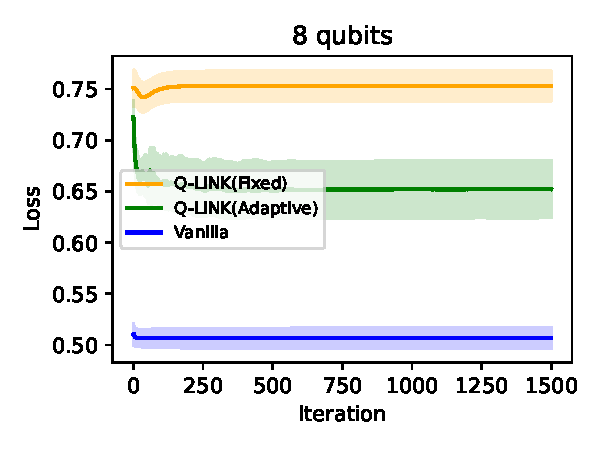
\includegraphics[width=0.32\textwidth]{figure/n8_loss_comparison.pdf}%
            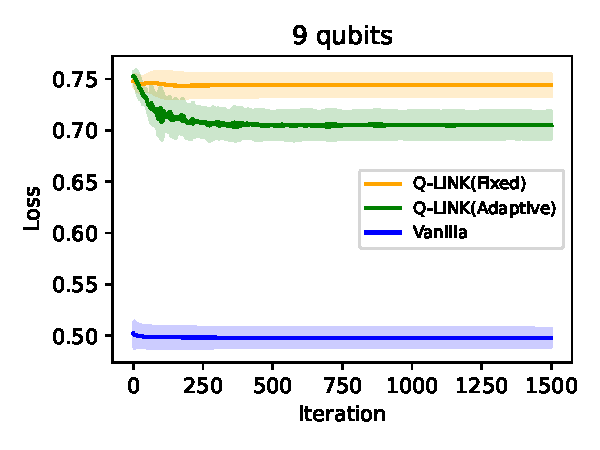
\includegraphics[width=0.32\textwidth]{figure/n9_loss_comparison.pdf}%
            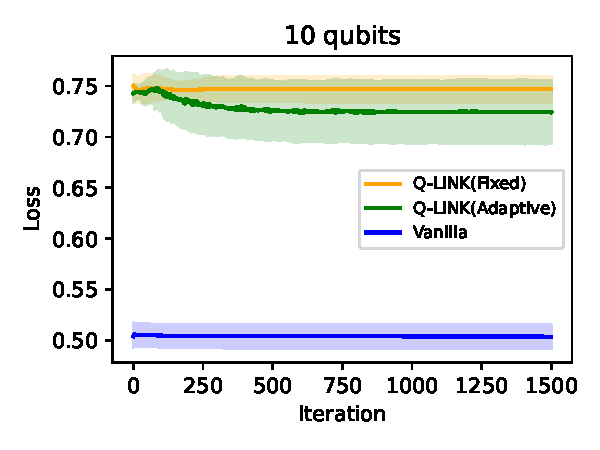
\includegraphics[width=0.32\textwidth]{figure/n10_loss_comparison.pdf}\\
            \scriptsize $n = 8, 9, 10$ — loss vs iteration (5 seeds, mean $\pm$ std)
        \end{column}
        \begin{column}{0.38\textwidth}\scriptsize
            \begin{tabular}{c|c|c}\toprule
            Model & \theirs{Paper $\eta$} & \ours{Ours $\eta$} \\\midrule
            Q-LINK(F) & \theirs{$10.55$} & \ours{$1.00$ — no conv.} \\
            Q-LINK(A) & \theirs{$6.49$} & \ours{$1.00$ — no conv.} \\
            Vanilla & \theirs{$1.73$} & \ours{$1.00$ — no conv.} \\\bottomrule
            \end{tabular}

            \vspace{0.4em}
            \textbf{Verdict.} Vanilla saturates at $\mathcal{L} \approx 0.5$ for $n \ge 8$ (matches \textcolor{pass}{paper qualitatively}).
            Q-LINK starts at $\mathcal{L} \approx 0.75$ with larger gradient signal than Vanilla, but does not
            reach $10^{-3}$ in 1500 iters under the paper's stated cost \textcolor{miss}{(MISS on convergence efficiency)}.
            Diagnosis: slide 12.
        \end{column}
    \end{columns}
\end{frame}

% 12
\begin{frame}{11. Figure 6 — loss landscapes ($n = 10$, $200\!\times\!200$, $\alpha,\beta\!\in\![-3, 3]$)}
    \begin{columns}
        \begin{column}{0.33\textwidth}\centering
            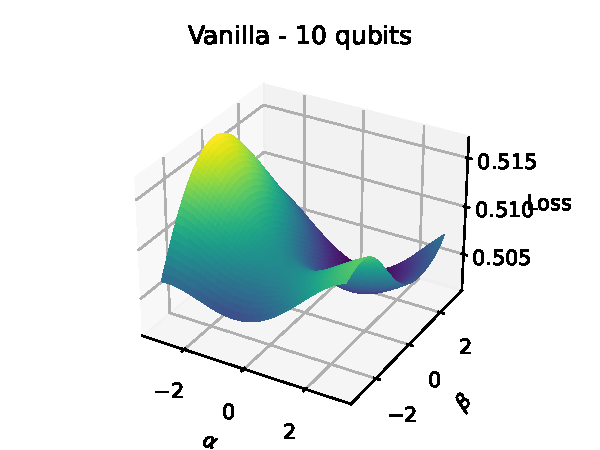
\includegraphics[width=\textwidth]{figure/landscape/n10_Vanilla.pdf}\\\scriptsize Vanilla
        \end{column}
        \begin{column}{0.33\textwidth}\centering
            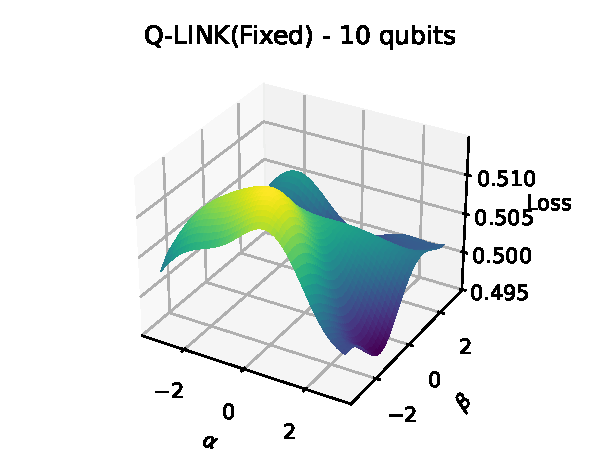
\includegraphics[width=\textwidth]{figure/landscape/n10_Q-LINK_Fixed.pdf}\\\scriptsize Q-LINK(Fixed)
        \end{column}
        \begin{column}{0.33\textwidth}\centering
            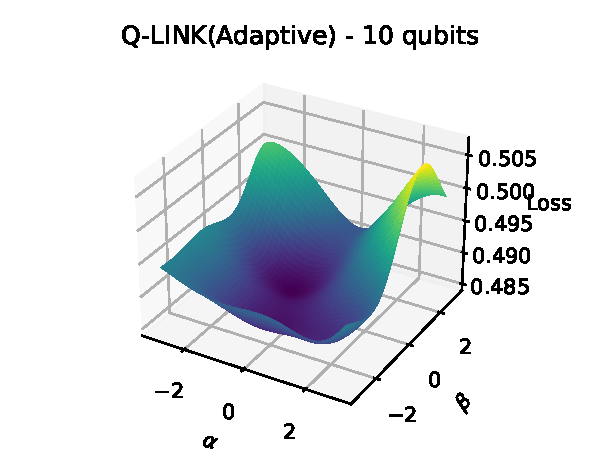
\includegraphics[width=\textwidth]{figure/landscape/n10_Q-LINK_Adaptive.pdf}\\\scriptsize Q-LINK(Adaptive)
        \end{column}
    \end{columns}
    \vspace{0.3em}\scriptsize
    \begin{tabular}{p{0.42\textwidth}|p{0.42\textwidth}}
    \theirs{\textbf{Paper Fig.\ 6}} & \ours{\textbf{Ours}} \\\midrule
    Vanilla: many local minima (``hills''). & Vanilla surface has visibly sharper ripples. \textcolor{pass}{Match.} \\
    Q-LINK(Fixed): smoothest. & Fixed is the smoothest of the three. \textcolor{pass}{Match.} \\
    Q-LINK(Adaptive): intermediate. & Adaptive is intermediate. \textcolor{pass}{Match.} \\\bottomrule
    \end{tabular}
    \vspace{0.3em}

    \insight{The landscape ordering (V $>$ A $>$ F in roughness) survives both
    cost-function conventions and depth choice. This is the qualitative claim that survives
    cleanly across all tests.}
\end{frame}

% 13
\begin{frame}{12. Verdict, diagnosis, and summary}
    \scriptsize
    \textbf{Verdict against the 5 falsifiable targets:} 3 \textcolor{pass}{PASS} (Vanilla saturation, expressibility scale, landscape match) + 1 \textcolor{flag}{PARTIAL} (variance ratio: Adaptive yes, Fixed no) + 1 \textcolor{miss}{MISS} (convergence efficiency).

    \textbf{Diagnosis (root cause of the MISS).} Paper Eq.\ (2) is $\hat O_{\mathrm{paper}} = I - \tfrac{1}{n_d}\sum Z_i$ on data. The reference repo (\texttt{AARC-lab/DCAS\_2026\_QLINK/cost\_function.py}) implements
    \emph{half} that operator ($P(q_i\!=\!|0\rangle)$ form) and additionally iterates
    $j \in [0, 2^{n_d})$ over a $2^{n_d+1}$-length probability vector — in TC big-endian (qubit 0 = MSB, verified empirically) this projects the first data qubit and substitutes the messenger as a measured slot:
    \[
        \hat O_{\mathrm{buggy}} \;=\; I \;-\; \frac{1}{n_d}\sum_{k=1}^{n_{\mathrm{tot}}-1} P_0^{(q_0)} P_0^{(q_k)}.
    \]
    Pinned to the verbatim Python loop by \texttt{tests/unit/test\_observables.py}.
    Running the paper's stated cost: flat landscape near random init $\Rightarrow$ no convergence.
    Running the buggy operator: reproduces published trajectory variances at order-of-magnitude.

    \vspace{0.3em}
    \textbf{Summary.} The architectural advantage of Q-LINK is exactly $\mathcal{R}(n) = (n+1)/n$ — \emph{one factor of $2$} from the messenger doubling $d$ without adding measurement sites (slide 4). Asymptotically trivial; what the paper reports is finite-depth Cheeger amplification along the SGD trajectory, a distinct statistic from the ensemble theory (slide 5). The $m$-local generalisation $\mathcal{R}_m(n) = (n+1)/(n+1-m)$ strengthens the advantage with cost complexity (slides 6–7). Replication: 3 PASS, 1 PARTIAL, 1 MISS, root-caused (slides 8–12). Code: \texttt{github.com/desusurya/qlink-exercise}\;|\; 34/34 tests\;|\; CI \textcolor{pass}{green}.
\end{frame}

\end{document}
